
%(BEGIN_QUESTION)
% Copyright 2012, Tony R. Kuphaldt, released under the Creative Commons Attribution License (v 1.0)
% This means you may do almost anything with this work of mine, so long as you give me proper credit

Calculus is believed to be inscrutable by many people.  Yet, anyone who has ever driven a car has an intuitive grasp of calculus' most basic concepts: {\it differentiation} and {\it integration}.  These two complementary operations may be seen at work on the instrument panel of every automobile:

$$\includegraphics[width=15.5cm]{i01560x01.eps}$$

On this one instrument, two measurements are given: speed in miles per hour, and distance traveled in miles.  In areas where metric units are used, the units would be kilometers per hour and kilometers, respectively.  Regardless of units, the two variables of speed and distance are related to each other over time by the calculus operations of integration and differentiation.  My question for you is, {\it which operation goes which way?}

We know that speed is the rate of change of distance over time.  This much is apparent simply by examining the units (miles {\it per hour} indicates a rate of change over time).  Of these two variables, speed and distance, which is the {\it derivative} of the other, and which is the {\it integral} of the other?  Also, determine what happens to the value of each one as the other maintains a constant (non-zero) value.

\vskip 20pt \vbox{\hrule \hbox{\strut \vrule{} {\bf Suggestions for Socratic discussion} \vrule} \hrule}

\begin{itemize}
\item{} The relationship of speed to distance traveled, as recorded by a speedometer/odometer, lends itself well to exploration through {\it thought experiments}.  Try using a thought experiment to explain the operation of an odometer in terms simple enough for someone who has never seen an odometer before to understand (a child, perhaps).  What does the odometer do when the automobile is traveling along at a constant speed?  What changes when the automobile's speed increases or decreases?  How does the speedometer needle position on the scale relate to the odometer's digits over time?
\end{itemize}

\underbar{file i01560}
%(END_QUESTION)





%(BEGIN_ANSWER)

Speed is the derivative of distance.  In other words, if the speedometer broke, we could calculate the vehicle's speed by differentiating the odometer's reading (distance traveled) with respect to time.

\vskip 10pt

Distance is the integral of speed.  In other words, if the odometer broke, we could calculate the distance traveled by integrating the speedometer's reading with respect to time.

\vskip 10pt

If the speed holds steady at some non-zero value, the distance will accumulate at a steady rate.  If the distance holds steady, the speed indication will be zero because the car is at rest.

%(END_ANSWER)





%(BEGIN_NOTES)

The goal of this question is to get students thinking in terms of derivative and integral every time they look at their car's speedometer/odometer, and ultimately to grasp the nature of these two calculus operations in terms they are already familiar with.










\vfil \eject

\noindent
{\bf Prep Quiz:}

Describe in your own words a practical, real-life example of {\it integration}. 

%INDEX% Mathematics, calculus: integral and derivative related to motion

%(END_NOTES)

